% REMEMBER: You must not plagiarise anything in your report. Be extremely careful.

\documentclass{l4proj}

    
%
% put any additional packages here
%

\usepackage{amssymb}% http://ctan.org/pkg/amssymb
\usepackage{pifont}% http://ctan.org/pkg/pifont
\usepackage{array}
\usepackage{pdfpages}
\usepackage{cleveref }
\newcolumntype{P}[1]{>{\centering\arraybackslash}p{#1}}
\newcommand{\cmark}{\ding{51}}%
\newcommand{\xmark}{\ding{55}}%

\begin{document}

%==============================================================================
%% METADATA
\title{Android Prescription Managament System}
\author{Alastair Innes}
\date{April 02, 2021}

\maketitle

%==============================================================================
%% ABSTRACT
\begin{abstract}
    Existing mobile phone applications for managing medication are available, but they fail to effectively solve every problem that is expected of such an application. MedApp is an application that offers a solution to this, providing functionality for medicine reminders, inventory management and administering medicine instructions to patients. 
\end{abstract}

%==============================================================================

% EDUCATION REUSE CONSENT FORM
% If you consent to your project being shown to future students for educational purposes
% then insert your name and the date below to  sign the education use form that appears in the front of the document. 
% You must explicitly give consent if you wish to do so.
% If you sign, your project may be included in the Hall of Fame if it scores particularly highly.
%
% Please note that you are under no obligation to sign 
% this declaration, but doing so would help future students.
%
%\def\consentname {My Name} % your full name
%\def\consentdate {20 March 2018} % the date you agree
%
\educationalconsent


%==============================================================================
\tableofcontents

%==============================================================================
%% Notes on formatting
%==============================================================================
% The first page, abstract and table of contents are numbered using Roman numerals and are not
% included in the page count. 
%
% From now on pages are numbered
% using Arabic numerals. Therefore, immediately after the first call to \chapter we need the call
% \pagenumbering{arabic} and this should be called once only in the document. 
%
% Do not alter the bibliography style.
%
% The first Chapter should then be on page 1. You are allowed 40 pages for a 40 credit project and 30 pages for a 
% 20 credit report. This includes everything numbered in Arabic numerals (excluding front matter) up
% to but excluding the appendices and bibliography.
%
% You must not alter text size (it is currently 10pt) or alter margins or spacing.
%
%
%==================================================================================================================================
%
% IMPORTANT
% The chapter headings here are **suggestions**. You don't have to follow this model if
% it doesn't fit your project. Every project should have an introduction and conclusion,
% however. 
%
%==================================================================================================================================
\chapter{Introduction}

% reset page numbering. Don't remove this!
\pagenumbering{arabic} 

\section{Motivation}

The management of one's medication is a time-consuming process, with a lot of planning needing to go into it. For example, an individual has to not only plan and remember to take their medication on time, but also they need to ensure that their medication inventory is sufficient and that they need to take prompt action to order more medication if they are required to continue taking it. This becomes increasingly challenging when someone needs to take multiple medications throughout the duration of a week. According to a study conducted by the NHS in 2016, 24 percent of adults in England had taken three or more different prescribed medicines. 

A mobile application that can manage user-defined medicines would be a solution to this problem. Such an application would provide a user with the ability to input details about medication that they have been prescribed, so that they can receive reminders on their device to remind them to take their medication on time. The application would provide the functionality of tracking the current supply of each medication, deducting the quantity of it upon the user taking a dose. Once the supply of a medication drops below a certain threshold, the user will start to receive notifications that prompt them to order a repeat prescription so that they do not run out of it.

People can also make use of an online calendar system to organise their schedule, so that they can be prompted to remember events that occur on a given day. If an prescription management system is able to interface with a user's online calendar, then this could potentially reinforce the adherence of following a medication schedule even further due to the benefits calendar usage provides for memory.

\section{Aim}

The aim of this project is to develop a new prescription management system for Android devices that ensures that users are prompted to take their medication on time and are provided with reminders to refill their medication supply before it runs out. The system will also interface with an external online calendar, so that users can view what medicine they need to take on a given day in relation to other events that they have organised in their calendar. 

\section{Summary}

This paper is structured as follows:
\begin{itemize}
    \item \textbf{Chapter 2} examines literature that explains the importance of applications that help enforce medication adherence and also how online calendar usage assists with memory. It also examines existing solutions to prescription managements, discussing their strengths and weaknesses.
    \item \textbf{Chapter 3} summarises the formation of requirements for the application, describing how they were obtained and then how they were prioritised.
    \item \textbf{Chapter 4} discusses the design process, describing the process of designing the user interface. It additionally discusses the architecture of the system, how it interacts with external services and how notifications should be delivered. 
    \item \textbf{Chapter 5} reviews the implementation process, outlining the software engineering processes used to support development, outlining the technologies used during development and describing the achievements of the implementation.
    \item \textbf{Chapter 6} evaluates the developed product, detailing the effectiveness of testing strategies and the results of usability and correctness testing.
    \item \textbf{Chapter 7} summarises the paper as a whole, providing an overall reflection on the project and examining any potential future work for the project.
\end{itemize}

%==================================================================================================================================
\chapter{Background}

In this chapter, we examine the background research regarding how medication applications support medication adherence and how the use of an online calendar helps to assist prospective memory performance. It also looks into existing prescription management applications and discusses what they do well and what their shortcomings are.

\section{Medication Adherence}

The lack of medication adherence has been determined to be a major global problem by the World Health Organisation \citep{sabate2003adherence}, leading to increased rates of mortality for nonadherent patients. \cite{bedell2000discrepancies} discovered a 76\% discrepancy rate between the medication that was prescribed and what medicines the patient actually took . Prior research indicates that there is an inverse relationship between the frequency of required medication doses and medication adherence as a whole, which means that patients who are undergoing polypharmacy are at particular risk of misadherence \citep{pasina2014medication}. This is a major concern for patients who need to take medication for chronic diseases, with these patients being required to take more than one dose of medication on a daily basis \citep{saini2009effect}. 

There are many reasons as to why a patient will not follow their prescribed medication routine, such as having the perception that the medication is not helping them. However, the most frequent reasons for non-adherence are a result of involuntary causes such as forgetfulness and a lack of understanding of medication instructions \citep{perez2019mobile}. The act of remembering to carry out a task in the future is a function of prospective memory, which is an ability that declines with age \citep{maylor1990age, Zogg2011TheRO}. 

A traditional method of ensuring medication adherence is the pillbox (Figure~\ref{fig:pillbox}), which is a box with seven compartments, each corresponding to a day of the week. This meant that a patient would place in each compartment the medication that they need to take on that given day \citep{schwartz2017pillbox}. Studies show that patients who utilise pillboxes tend to exhibit greater levels of medication adherence, meaning that they are an effective solution to enforcing adherence \citep{e2013descriptive}. 

\begin{figure}[!ht]
    \centering
    \includegraphics[scale=0.85]{images/pillbox.jpg}
    \caption{Physical pillbox given to patients to help them adhere to medication schedules
        \newline Credit: https://www.dreamstime.com/photos-images/pillbox.html}

    \label{fig:pillbox}
\end{figure}

A modern method that is commonly used to remind people to carry out tasks is to receive reminder notifications on a smartphone. In the United Kingdom, 84\% of adults own a smartphone, meaning that adoption of the technology is widespread \citep{matthewboyler}. This suggests that developing an application that enables patients to setup their medication taking regime so that they can receive reminders to take their medication on time could potentially be a solution to improve medication adherence. Studies have been conducted to evaluate the effectiveness of medication reminder applications in improving medication adherence in comparison to traditional methods such as pillboxes, and in general they are a more effective method of preventing patients from forgetting to take their medication \citep{perez2019mobile}.

\section{Online Calendar Usage}

Human-computer interaction literature has a long history of studying calendar usage, predating the advent of digital calendars. It is under the field of Personal Information Management (PIM), which is concerned with how people manage their own information space. Calendars are typically used to support prospective memory, providing a system that people can refer to so that they can rememeber what they have scheduled in the future. From a survey conducted on Microsoft employees, 51\% of participants claimed to use their digital calendar for work and  personal events \citep{brush2005survey}, indicating that digital calendar usage is wide-spread. 

One of the most characteristic aspects of online calendars is that they can provide reminders for events added to the calendar, typically through app notifications and in some cases through email or SMS. For example, a user may insert an event into their online calendar to remind them that they have a dental appointment, setting the time period before the event occurs of when they would like to receive a reminder for the event. Google Calendar (Figure~\ref{fig:googlecal}) is one of the most popular online calendar services, with 25\% of mobile calendar users using it for planning their day \citep{ecal_2020}. A users Google Calendar is directly connected to their Google account, meaning that their calendar is shared across all of their devices.  

Studies have shown that the usage of Google Calendar has lead to enhanced performance of prospective memory, due to the cross-platform access to the calendar and the reminder systems put into place \citep{el2017google}. This therefore suggests that a medication reminder application that can sync medication taking events with a user's Google Calendar would help to further reinforce the adherence of taking medication by its further enhancement of prospective memory.    

\begin{figure}[!ht]
    \centering
    \includegraphics[scale=0.25]{images/googlecal.jpg}
    \caption{A desktop view of Google Calendar}
    \label{fig:googlecal}
\end{figure}

\section{Existing Applications}

There are many existing medication management applications on the Google Play Store for Android devices. This section will go into detail about the strengths and weaknesses of these applications, to ultimately come to a conclusion about what is missing from them as a whole. A summary of the applications that will be discussed in this section is located in~Table \ref{tab:appcomparison}.

\subsection{Medisafe}

Medisafe one of the most popular medicine management applications on the Play Store, with over one million downloads. It provides all of the essential features one would expect from a medication management app, enabling users to set-up their medication taking routines and receive notifications to remind them to take their medication.

Medisafe also provides multi-user use-cases, with the ability to allocate "Medfriends", who are an elected family member or friend who the user shares their medication taking routine with so that they can see if the user has taken their medication on time or not. Other multi-user features it has are setting up dependants so that the user can define medication for people that they care for and also the ability to send a status report to a carer via email so that they can examine the user's medication taking routine, so that they can check that the user has been adhering to their medication.

One feature that Medisafe does not have is the integration with an external calendar app, as it only uses its own internal calendar. This means that they cannot use one PIM system to manage their day, as they will need to use Medisafe to view their medicine taking schedule, meaning that it is difficult to directly compare this schedule to events that they have scheduled in their own online calendars. 

Medisafe also does not have the ability for the app to automatically register that they have taken their medication for them. It is possible that some users might not be concerned with registering with the app that they have taken their medication on time, but are only interested in knowing when their medication supply is running low. This means that this user has to still manually register with the app that they have taken their medication for the stock functionality to work accordingly, which is detrimental to their experience. 

\subsection{MyTherapy}

MyTherapy is another popular application for managing prescriptions for Android devices. It allows for users to setup their medication taking regime and receive notifications for doing so, and like Medisafe it also supports the tracking of medication stock levels so that a user can be notified when their stock becomes low. MyTherapy also provides users with the functionality to share their progress with their medication taking regime with a carer, which is done through the sharing of a verification code that enables the carer to enter into their own MyTherapy app so that they can begin viewing their patients progress. Unlike Medisafe, MyTherapy does not have the ability to directly setup medications for a dependent, as it is designed for a single user registering their own medication adherence. 

The notifications that are prompted from MyTherapy to remind users to take their medication are intrusive, with the notification locking up the users screen until they take action on it. This is beneficial as it forces the user into making a decision about taking their medicine, which helps improve adherence, but from a user experience point of view notifications like this can often be a result of frustration. According to a study conducted by \cite{vanneldas_2020}, unwanted notifications are one of the main factors that lead to people uninstalling apps, with 71\% of survey participants citing this as a reason they uninstalled apps. This emphasises the importance of having notifications that are non-intrusive and that are wanted by the user.

MyTherapy also fails to provide a connection to an external online calendar, meaning that all medication taking events are centralised within the one application. Additionally, it lacks the functionality for offering a user with the option to not have to manually register that their medication has been taken every time.

\begin{figure}[!ht]
    \centering
    \includegraphics[scale=0.30]{images/mytherapy.jpg}
    \caption{Example of MyTherapy's intrusive notifications}
    \label{fig:mytherapy_notif}
\end{figure}

\subsection{Medlist Pro}

Medlist Pro is a prescription management application that is designed for carers looking after patients. It allows for a carer to manage the medication of multiple different patients, by providing details of the medication that they need to take. However, the application as a whole does not have the greatest user interface, as it outdated and it is non-intuitive in regards to understanding how a user is to access certain parts of the application, due to the poor implementation of navigation elements.

The application attempts to manage medication stock by asking the user to provide the date of when they are to finish taking the medication. This is a rigid system which is flawed as a user could lose some of their medication by mistake. It also does not provide any sort of reminder that the medication is running low on supply. This highlights the need for a dynamic method of setting medication supply, which can account for the user making mistakes. There is also no aspect of registering that medication has been taken on time or not, meaning that this app only serves as a reminder system, meaning that Medlist Pro does not enforce adherence. 

\begin{figure}
    \centering
    \includegraphics[scale=0.4]{images/medlistpro.jpg}
    \caption{MedList Pro's User Interface}
    \label{fig:medlist_pro}
\end{figure}

\subsection{Pill Time Medication}

Pill Time Medication is another prescription management application that offers users to receive reminders to take their medication. The method of adding medication to the application is different from the rest of the apps in the market, as it requires that the user scans the barcode of their medication before adding details about their dose regime. This approach has some benefits, in particular it would assist users who have problems with their eyesight to setup their medication in the app. However, there is always the possibility that users might not have the original packaging of their medication on hand, meaning that they are essentially prevented from actually using the app.

Whilst Pill Time Medication's medication setup system fails to be a suitable solution for prescription management, it does emphasise the importance of ensuring the app is accessible for elderly users, especially because eyesight begins to deteriorate as people age \citep{salvi2006ageing}.

\subsection{Existing Applications - Conclusions}

By examining the most popular apps in the market, it is clear that as medication adherence solutions they are effective, but they are lacking additional features that can help reinforce this behaviour. As can be identified in Table~\ref{tab:appcomparison}, no popular app in Google Play provides the functionality for the user to synchronise their medication taking schedule with their online calendar, meaning that they cannot compare their intended medication routine with other events that they have planned. They also lack the functionality for users who are only interested in the management of medication stock levels, as these users are still required to automatically register that they have took their medication at the appointed time and will receive unwanted notifications reminding them to do so. Additionally, the case made from MyTherapy and its intrusive notifications highlights the importance of having notifications that are not noisy so that users do not become dissatisfied with their experience of the system.

\begin{table}[!ht]
    \centering
    \caption{Table that displays what functionality existing prescription management applications have}
    \begin{tabular}{ | P{3.3cm} | P{2cm}  P{2cm}  P{2cm}  P{2cm} | }
        \hline
         & & & & \\
        \textbf{Application Name} & Medisafe &  MyTherapy & Medlist Pro & Pill Time Medication \\
         & & & & \\
        \hline
         & & & & \\
        \textbf{Application Features} & & & &   \\
         & & & & \\
        \hline
         & & & & \\
         Dose Reminders & \large{\cmark} &  \large{\cmark}  &  \large{\cmark}  &  \large{\cmark}  \\ 
         & & & & \\
        \hline
         & & & & \\
         Stock Management & \large{\cmark} &  \large{\cmark}  &  \large{\cmark}  &  \large{\xmark} \\
         & & & & \\
        \hline
         & & & & \\
         Refill Reminders & \large{\cmark} &  \large{\cmark}  &  \large{\cmark}  &  \large{\xmark} \\
         & & & & \\
        \hline
         & & & & \\
         Manage Dependents & \large{\cmark} &  \large{\xmark}  &  \large{\cmark}  &  \large{\xmark} \\
          & & & & \\
        \hline
         & & & & \\
         Carer Connectivity & \large{\cmark} &  \large{\cmark}  &  \large{\cmark}  &  \large{\xmark} \\
         & & & & \\
         \hline
         & & & & \\
         Intrusive Notifications & \large{\xmark} &  \large{\cmark}  &  \large{\cmark}  &  \large{\xmark} \\
          & & & & \\
        \hline
         & & & & \\
        Barcode Scanning & \large{\xmark} &  \large{\cmark}  &  \large{\xmark}  &  \large{\cmark} \\
         & & & & \\
        \hline
         & & & & \\
        Automatic Taking & \large{\xmark} &  \large{\xmark}  &  \large{\xmark}  &  \large{\xmark} \\
         & & & & \\
         \hline
          & & & & \\
         Calendar Integration & \large{\xmark} &  \large{\xmark}  &  \large{\xmark}  &  \large{\xmark} \\
          & & & & \\
        \hline
    \end{tabular}
    \newline
    \label{tab:appcomparison}
\end{table}



%==================================================================================================================================
\chapter{Requirements}

This chapter provides detail on how the method as to how requirements for the system were gathered, and subsequently explains how they were prioritised for development.  

\section{Requirements Acquisition}

\subsection{User Personas}

To elicit requirements for this application, user personas were created to conceptualise the different kinds of users that would use the application. Each persona outlined who the person is, what their motivation for using a medication management system and ultimately made clear what features they would require from such a system. Developing user personas for health care technology is beneficial as it enables the characterisation of elderly users and identify their needs as users \citep{lerouge2013user}. This is important, as elderly users tend to take medication more frequently and have worse memory, so the app must be tailored to fit their needs.

Figure 3.1 demonstrates some of the user personas that were generated for this application. These encompassed a wide variety of different types of people who would want to make use of a prescription management application, and explored exactly what they would require from such an application.

\begin{figure}[!ht]
    \centering
    \includegraphics[scale=0.6]{images/user-personas.png}
    \caption{Examples of the user personas designed for eliciting requirements}
    \label{fig:my_label}
\end{figure}

\subsection{User Stories}

After forming the user personas, this lead to deriving user stories that represented the needs for users of the app. It was clear that there were two different types of possible types of user of this app; either a patient who has been prescribed medication and is looking to manage it on their own, or an individual who has a duty of care for another person and wants to manage their medication for them. For the sake of brevity, the requirements for a patient are also requirements for a carer. 

\subsubsection{Patient User}
\begin{itemize}
    \item As a patient, I want to be able to register the medication that I take with a system that gives me reminders to take my medication, so that I do not forget to take it and that I can take it on time.
    \item As a patient, I want to be able to receive advance warning that my medicine is running low, so that I can reorder my prescription and receive it on time.
    \item As a patient, 
    \item As a patient, I want to connect the medication information I have registered with the app with an online calendar, so that I see where my medicine taking regime fits in with the rest of my day.
\end{itemize}
\vskip 1em
\subsubsection{Carer User}
\begin{itemize}
    \item As a carer, I want to be able to manage the medication of multiple patients at once through the use of an app, so that I can keep track of 
    \item As a carer, I want to be able to share with patients their medication routines, so that they know what medicine they need to take and when. 
    \item As a carer, I want to be able to see a log of a patients medication taking history so that I can identify if there are any issues. 
\end{itemize}

\section{Functional Requirements}

\subsection{Requirements Questionnaire}

After creating user stories, it was decided to conduct a questionnaire with potential end-users to help validate the priority of the stories. The survey provided gave a list of nine different features for a medication app, alongside the context of how said feature would work, with participants asked to rank each one from 1 to 5 based on how important they believed the feature to be for a medication app, with 1 being that they viewed the feature as very unnecessary and 5 being that they think the feature is very important. The features asked about were as follows:
\begin{enumerate}
    \item Notifications to take medication;
    \item Keeping track of stock;
    \item Reminders for low stock;
    \item Integration with Google Calendar;
    \item Different profiles for medication;
    \item Scanning barcodes for adding medication;
    \item Selecting specific medications to synchronise with Google Calendar;
    \item Login via multiple devices;
    \item A log of medication.
\end{enumerate}

Twenty responses were received from the survey, yielding some useful results (\ref{fig:req1results}-\ref{fig:req9results}). In general, the respondents deemed each requirement to be of somewhat importance, but some proving to be absolutely vital. By inspecting the mean scores of each feature (Figure~\ref{fig:mean_requirements}), it can be seen that on average that more respondents seen the features that incorporated carer functionality to be less popular, alongside the scanning barcodes to add medication. Some participants provided an explanation as to why they selected the option, with one participants claiming that the ability to assign medication for other people is "not very useful for me, but a life save for others" (Appendix ~\ref{fig:req5results}). As this was one of the lowest-scoring features overall, and that other apps such as Medisafe and MyTherapy already provide this functionality, it was decided that this app will focus on the experience of a single patient user. 

\begin{figure}[]
    \centering
    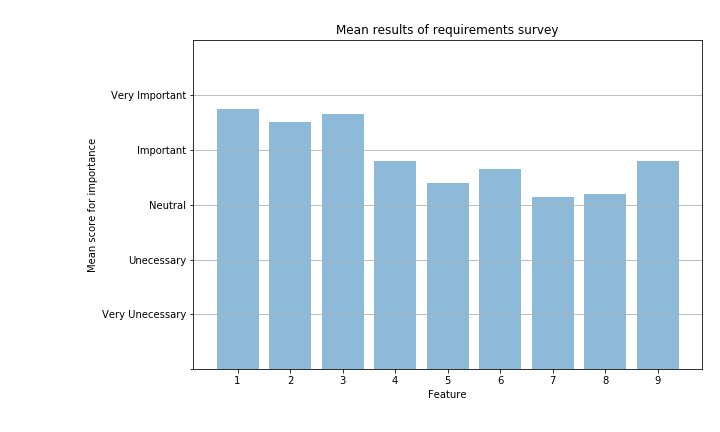
\includegraphics[scale=0.6]{images/requirementssurvey/medapprequirements.png}
    \caption{Mean score of the requirements survey}
    \label{fig:mean_requirements}
\end{figure}



\subsection{Requirements Prioritisation}

Following the completion of the requirements survey, the next stage was to formalise these into functional requirements that defined the features that are expected to be in the application, and assigned their priority for development. The MoSCoW prioritisation technique \citep{waters2009prioritization} was used to label each requirement based on how important they are for the product. This splits the requirements into four groups; Must Have for mandatory requirements, Should Have for important requirements that provide significant value, Could Have for requirements that have a limited impact if they are not completed and Won't Have for requirements that would be nice to have, but are outwith the scope of the project.


\vskip 1em
\subsubsection{Must Have}
\begin{itemize}
    \item An Android application to manage prescriptions.
    \item The ability to create, remove, update and delete medicine registered to the app.
    \item Be able to provide reminders to take doses of medication at appointed days and times.
    \item Allow users to register that they have taken medication, which would deduct from the stock of that medication.
    \item Allow users to define how many days in advance of a medicine running they would like to start receiving reminders to order more.
    \item The option to connect the app to a user's Google account, so that 
\end{itemize}

\vskip 1em
\subsubsection{Should Have}
\begin{itemize}
    \item The ability to disable notification for taking medication reminders and/or refill reminders.
    \item The ability for users to be able to view a log of their activity in the app; for both their medication taking history and for their medication refill history.
    \item The option to enable the automatic taking of medication, so that the user does not need to register that they have taken their medication each day.
    \item The user should be able to alert the application that they have requested a new prescription for a medication, so that they do not need to constantly receive refill reminders when they have already taken action regarding them.
\end{itemize}

\vskip 1em
\subsubsection{Could Have}
\begin{itemize}
    \item Offering the user the ability to rectify failing to register with the app that they actually took their medication on time, by enabling them to inform the app that they actually have done so.
    \item A remote backend database for the storage of medication information, meaning that a user would be able to register an account for the application and to 
    \item Ability to connect with other users and act as their carer, essentially taking over the management of their prescriptions for them.
    \item Provide a graphical visualisation of medication refill history in the form of a chronological line graph. 
\end{itemize}

\vskip 1em
\subsubsection{Won't Have}
\begin{itemize}
    \item The functionality for users to use their device's camera to scan the barcode of their medication, so that they can automatically add details of the medicine to the application without having to manually do so
\end{itemize}

\section{Non-functional Requirements}

Non-functional requirements are requirements of the application that are not in relation to the features that the app must have, but instead they are in regard to criteria that can judge the operation of the app. These requirements are as follows:
\vskip 1em
\begin{itemize}
    \item The app must be have a clear and understandable user interface so that it is usable. Particularly, as older users are more likely to be using this app due to their tendency to be taking more medicine, meaning that the user interface must be suitable for them.
    \item The app must deliver notifications reliably, because if it fails to do so then individuals might forget to take their doses of medication on time. As people age they tend to exhibit cognitive decline in their ability to remember, meaning that the prompt arrival of reminders is of upmost importance to ensure prescription adherence. 
    \item Because users might regard information about their medication taking history as sensitive, the storage of this information must be kept secure and maintained accordingly. The app should also aim to 
    \item The app must also obtain user consent to use certain permissions to enable Google Calendar integration. This is vital as information about a user's medication could be considered sensitive to them and they may not be willing to share this information with a Google service.
\end{itemize}

%==================================================================================================================================
\chapter{Design}

This chapter outlines the design stage of the development process. It explains how concepts for the user interface were generated and put into fruition, to then go into detail about the architecture of the application. This chapter will also explain how the app will interact with the external Google Calendar API and will demonstrate the design considerations taken for the notifications that will be produced by the app.

\section{User Interface}

As stated in Section 3.3., it was important that the application has an understandable user interface that is easy to use for a wide range of users, in particular for untrained and elderly users. To generate concepts for this, the process of wireframing was used, which is a technique that is used to design an application at a structural level. In particular, wireframes will demonstrate interface components for key pages of an application, so that the interaction with them can be conceptualised \citep{rees}. This is advantageous, as this process can help to identify problems with the usability of the app before starting the implementation of it, resulting in less time being spent trying to fix usability problems during implementation \citep{snyder2003paper}.  

The first stage of wireframe generation was to draw out some simple paper prototypes. These were essentially just simple sketches of an example medication application on a mobile device, giving a simplistic overview of what it would possibly end up looking like. The main interaction outlined by the paper prototypes was that of the app navigation, utilising a bottom navigation bar for navigating between app components and a floating action button that is to perform the primary function of the app, which is to add medication. Additionally, the home page of the app has a list of cards, with each individual card representing a dose of medication that the user has to take.

The act of sketching paper prototypes was beneficial, as it enabled the rapid generation of different user interface concepts, which was beneficial as it allowed for a variety of different design concepts to be produced within a short time frame. For example, during the creation of paper prototypes, it was apparent that there should not be an explicit requirement to sign into the system every single time to start using it, as a user would want to quickly access the app and register that their medication has been taken. This lead to this design choice being discarded in the future iterations of the user interface design.

\begin{figure}[]
      \centering
      \includegraphics[scale=0.6]{images/paperprototypes.jpg}
      \caption{Final paper prototypes}
      \label{fig:Final paper prototypes}
\end{figure}
\newpage

Following the finalisation of paper prototypes, a computer generated low-fidelity prototype of the application was then created using the Balsamiq Wireframes tool. Balsamiq enabled the creation of interactive prototypes, meaning that you could click on user interface components and then the prototype would dynamically change based of the interaction, mirroring what would be expected in an actual application. This was particularly useful, as it conceptualised how the user interacts with the system, allowing for usability faults to be identified before carrying them over to the implementation. The first set of refined prototypes for the app are located in Appendices~\ref{fig:prototypes1}-\ref{fig:prototypes12}.

One of the design issues raised during the evaluation of the initial set of refined prototypes was that there was no real defined method of assigning the medication frequency, as it was based off the assumption that every medication would be taken once every day. To account for this, a new set of refined wireframes were developed to demonstrate how a user would register how many doses of a given medication they need to take and how frequent they need to take it. This was split into three options: \
\begin{itemize}
    \item \textbf{Daily} for medications of which the dose needs to be taken on a daily basis;
    \item \textbf{Weekly} for medications where the dose is only required to be taken once a week;
    \item \textbf{Custom} for medications that need to be taken on appointed days of the week, for instance a medication that only needs to be taken on Monday and Wednesday.
\end{itemize}

The refined prototypes for this process are located in appendices (INSERT APPENDENCIES HERE!)


\newpage
\section{Google Calendar API}

For a mobile application to be able to make changes to an individuals Google Calendar, it needs to make use of the Google Calendar API. The API works through a client library by making HTTP calls to a backend that can create, update and delete events in a user's Google Calendar. To access a Google API, the OAuth 2.0 protocol is used for user authentication and authorisation \citep{hardt2012oauth}. This protocol is designed to allow users to share certain data with an application while keeping their personal information such as usernames and passwords secret. In our case, MedApp should be able to make changes to a user's Google Calendar using OAuth 2.0 without knowing any personal details about the user.

To utilise the Google Calendar API, the app must first register with the Google API Console to obtain OAuth 2.0 credentials. Then the application must obtain an access token that grants access to the API, which requires the user to log in with their Google Account and provide consent for API permissions, in this case the permissions the user has to consent to are the editing of their Google Calendar. Upon the user agreeing to the permission, the access token is sent to the application from the Google Authorisation Server, accompanied with a list of scopes of access that has been granted by the token. Once this process is complete, the app can now make API calls to make changes to the user's Google Calendar, by sending the access token to the Google Calendar API in an HTTP Authorisation Header to the API endpoint. Figure~\ref{fig:googlecalapiauth} shows a visual representation of how the application makes use of the OAuth 2.0 protocol to call the Google Calendar API.


\begin{figure}[!ht]
    \centering
    \includegraphics[scale=0.7]{images/googlecalapi.jpg}
    \caption{Diagram demonstrating how MedApp uses the OAuth 2.0 protocol to gain access to the Google Calendar API upon the user providing consent.}
    \label{fig:googlecalapiauth}
\end{figure}

The events that will be added to a user's Google Calendar from the app will be directly related to the medication that they have added to the app. For each medication, there will be an event for a refill reminder, an event for when the medication is empty, and an event for each dose of the medication the user is to take. These events should be updated dynamically according to changes made to medication within the app by the user, for example the recurrence of the dose reminders and the dates of the empty and refill events will be updated when the user refills their medication in the app, and the events relating to a medication are removed from Google Calendar if the user deletes the medication from the app. The actions of a user and the corresponding action in their Google Calendar is pictured by Table \ref{tab:googlecal}.

\begin{table}[!ht]
    \centering
    \caption{Table that demonstrates how a user's action in MedApp will effect their Google Calendar}
    \label{tab:googlecal}
    \begin{tabular}{|P{6cm}|P{6cm}|}
        \hline
        \textbf{User action in MedApp} & \textbf{Google Calendar API Response} \\
        \hline
        & \\
        \hline
        & \\
        User signs in to Google in MedApp & Events for each medication in MedApp are added to Google Calendar \\
        & \\
        \hline
        & \\
        User signs out of Google in MedApp & Events for each medication in MedApp are deleted from Google Calendar \\
        & \\
        \hline
        & \\
        User adds new medication to MedApp & Events for that medication in MedApp are added to Google Calendar \\
        & \\
        \hline
        & \\
        User deletes medication from MedApp & The events relating to the deleted medication are deleted from Google Calendar \\
        & \\
        \hline
        & \\
        Users updates quantity of medication in MedApp & The corresponding events in Google Calendar are updated \\
        & \\
        \hline
    \end{tabular}
\end{table}

 
\section{Database Structure}

Once the design of the user interface was completed, the structure of the backend database was then considered. There are too main entities in a medication taking app; the actual medication itself and the doses of which a patient has to take of it. A patient may be required to take multiple doses of a medication a day, or wish to take it at different times of the day on different days, meaning that there is a one-to-many relationship between a medication and its doses. A medication will also have log events that correspond to events for taking medication and for refilling medication. This will also be a one-to-many relationship between the medication and its log events in the database schema.

A medication is made up several attributes; the name of the medication, the current quantity the patient has of the medication, the form of which the medication is taken in (for example, a medication can be taken in the form of a pill) and the strength of the active ingredient in the medication. The medication will also have attributes that determine if the user has selected for the medication to be taken automatically by the system or if the user has registered to the app that they have requested a refill.

A dose of medication is made up of the time of which the dose is supposed to be taken so that they can be notified for it, the frequency determining how often the dose has to be taken in a week and how much of the medication is supposed to be taking for this given dose. The user will need to register with the app that they have taken this dose, so that the quantity of the medication can be reduced accordingly, so there must also be an attribute representing if this has occurred or not. However, if the medication that the dose instance is related to has been selected to be taken automatically taken by the system, the user will not need to register that the dose has been taken and thus the system will deduct the stock accordingly at the end of the day. Each dose must be updated on a daily basis to set the dose instances for that day to be registered as not taken. 

Additionally, if the user has decided to allow the application to synchronise their medication regime with their Google Calendar, then there must be a unique identifier to the corresponding events. This is so that when the user makes changes to a medication within the app, then the Google Calendar API can identify the respective events and update them accordingly. Each Google Calendar event has a unique string id, meaning that when the event is first created its id must be retrieved and stored by the application. Therefore, each medication must have attributes that records the ids of the medication empty event and the refill reminder event, and each dose must have an attribute that stores the id of the respective dose taking event from Google Calendar.

\section{Notification Design}

The design of the notifications coming directly from MedApp was carefully considered to try and ensure that they are as non-intrusive as possible. There will be two types of notification that MedApp will provide; notifications to remind users to take their medication, and notifications to alert users that their medication supply is running low and they need to order a refill.

For the medication taking reminder, this notification should inform the user what medication it is they need to take, and what quantity of it should be taking at the given time. Unlike MyTherapy's full-screen notifications, the notification received will be a simple drawer notification. When the user presses the notification, they will be taken to the home page of the app where they can register that they have taken the dose. However, the user will be able to take the medication from outside the app by pressing the "Take" action button in the notification. This is an important option, as it provides the user with the option to be able to register that their notification have been taken without having to actually go into the app, meaning that the system has less friction to use. If a user has opted for their medication to be taken automatically, then they will not receive any notifications to remind them to take their medication.


\begin{figure}[!ht]
    \centering
    \includegraphics[scale=0.7]{images/notifications/dose_reminder.png}
    \caption{Concept for the dose reminder notification}
    \label{fig:dose_notification}
\end{figure}
\newpage
The design of the refill reminder is similar to the medication taking reminder in design. When a medication hits a user-defined number of days until the supply runs out, the user will start to receive a reminder that they need to refill their medication. This reminder will occur daily until either the user refills their medication supply, or they register with the app that they have requested a refill. Clicking the notification will take the user to a page where they can refill the medication. 

\section{Design - Summary}

This chapter provided an abstract overview of the design of the application. It detailed the process of designing the user interface and what design choices were made for it, it examines how the Google Calendar API will be utilised to allow MedApp to share a user's medication information with their Google Calendar, it discusses how the database will be structured and how and where notifications will arise.

%==================================================================================================================================
\chapter{Implementation}

This chapter provides detail about the implementation of MedApp, detailing the software engineering processes that were used to support development, describing the technologies used for development and what has been achieved by development. 

\section{Development Tools}

To create the application, the Android Studio Software Development Kit (SDK) was used, which is a collection of software development tools for creating Android applications. The Android Studio IDE is a powerful IDE that bundles the SDK with it for development. The IDE is based on Jetbrains' IntelliJ IDEA, meaning that it not only has all of the benefits that IntelliJ has, it also has Android development specific features to aid the productivity of development. This included an emulator of an Android device, which was beneficial as it meant that the app could be tested on a variety of different devices of varying screen sizes.

As Android Studio is used to create applications that are native to the Android operating system, the native language of the operating system is used to build the application, which is Java. This access to the operating system is beneficial as it enables the app to be able to perform operations such as pushing notifications directly from the app. For hybrid app development solutions such as Flutter, notifications can only be pushed from requests being made to the operating system from backend databases like Firebase. This means that for notifications to be received from a hybrid app, then the user would need to maintain an Internet connection. As a consequence, receiving notifications from a native application is more reliable than hybrid applications, which is of importance to this application as reminder reliability is essential to ensuring medication adherence.

Since the app would be a native app, this meant that there was no requirement to setup an external backend database to store user medications. Instead, a local SQLite database was used to manage the storage of the user's medication. This was a good solution, as it was very lightweight and it typically results in better performance. It is also well-suited for an app that is for designed for the use of a single user, which is what this app prioritised over multiple users. 

\section{Version Control \& Continuous Integration}

To ensure high quality development, continuous integration was utilised. As GitLab was the choice of repository, it meant that not only was code continuously backed up in an appropriate location, it also meant that GitLab's continuous integration functionality could be used. GitLab provides public access to GitLab runners, which enables jobs to run in a pipeline to perform the continuous integration.

Two stages of continuous integration were used for this project; the first to build the app and check that the code passed a quality test, and the second to perform unit tests on the app. The build stage ensures that the code committed will  compile and creates an APK file which can be downloaded on an Android device to run the app if it does compile. Concurrently, the linting job will take place to ensure that the code committed into the repository will not break any user interface components on an Android device.

The use of continuous integration was successful for the build stage, but was redundant for the testing stage. This was because that the unit tests that were created for this application were instrumented unit tests, which could not be run on the public GitLab runner due to it not being able to run them on an Android devices. There are alternatives solutions that could have been used in order to perform automated testing for the application, for example utilising the Firebase Test Lab, but it was decided that this would not be a priority and instead tests will be executed manually.

\section{Google Calendar API}

To implement the Google Calendar API, the user must first authenticate their Google Account with MedApp. To do this, they need to sign in with their Google account in the settings page and authorise MedApp to read and make changes to their Google Calendar. Doing this grants MedApp the API token required to make changes to the users Google Calendar, as detailed in Figure \ref{fig:googlecalapiauth}.

The main thread of an Android application is a user interface thread, which meant that it was impossible to make requests through the network to make API calls. 

One of the problems faced during the development of Google Calendar synchronisation was that when too many API calls were being made at once, then occasion

\lstset{language=Java}
\begin{figure}[!ht]
    \centering
    \begin{lstlisting}
    public void googleCalendarAPICall(int depth) {
        try {
            apiCall();
        }
        catch (ApiException e) {
            // Only allow a limited number of attempts
            if (depth < 7) { 
                long backoff = (long) Math.pow(2, depth) * 10; 
                Thread.sleep(backoff);
                googleCalendarAPICall(depth++);
            }
        }
    }
\end{lstlisting}
    \caption{Generic version of the exponential backoff algorithm utilised for Google Calendar API calls}
    \label{fig:exponential_backoff}
\end{figure}

\section{Carer Functionality}

Since there was time remaining for the implementation of the application, it was decided to try and implement some sort of multi-user functionality. Since the choice of database meant that it was difficult to share medication through the app itself, the use of the Google Calendar connectivity offered an alternative approach. In Google Calendar, it is possible to invite event attendees to an event, meaning that if the invitee has a Google account then they are able to see an event that they have been invited to on their own Google Calendar. 

This brought forward the idea of being able to select a patient from their contacts when adding a medication to share with them the Google Calendar events for taking their medication. The Google People API was used to be able to retrieve contacts from a users Google contacts, using the same authorisation process as the Google Calendar API. When finalising a dose, 


%==================================================================================================================================
\chapter{Evaluation} 

The chapter specifies the methods used to evaluate the implemented application. In particular, the evaluation methods employed are unit testing to ensure correctness of the application and a user evaluation. The outcomes of these processes will be analysed to evaluate MedApp. Finally, the requirements of the project will be examined to find out if they have been met adequately.

\section{Unit Testing}

To test the correctness of MedApp, unit tests were created to validate that the system performed as expected. Tests were created to verify that database operations performed as expected, ensuring that events that are supposed to occur at certain times actually happen, and also validating the users interaction with the user interface. The tests implemented were instrumentation tests, meaning that they had to be ran on an Android device and could not just use the Java Virtual Machine to do so. The testing library used was Espresso, which is a native framework developed by Google for the automated testing of Android applications. Espresso is similar in nature to the automatic web application test suite Selenium WebDriver, except that it is for Android apps on an Android device instead of a web application in a web browser. 

In order to produce a report on the coverage of the unit testing that was conducted, the JaCoCo toolkit was used, which is pictured in Figure \ref{fig:jacoco}. This report shows that the tests achieved a line coverage of 73\% and a branch coverage of 48\%. This was good coverage overall, but was not complete as it proved to be challenging to test the correctness of the Google Calendar functionality. This would have required the creation of mock Google services, a mock Google user, and a significant amount of editing existing code to support the tests, meaning that the amount of development time required to validate the correctness of this functionality would take too long to complete. However, manual testing will be conducted to confirm that the Google Calendar synchronisation works as intended.


\begin{figure}[!ht]
    \centering
    \includegraphics[scale=0.9]{images/testcoverage.png}
    \caption{Code coverage report illustrating a line coverage of 73\% and a branch coverage of 48\%}
    \label{fig:jacoco}
\end{figure}
\newpage

\section{Google Calendar - Manual Testing}

Due to the challenge of writing unit tests to test the Google Calendar API functionality of the app, a manual approach was taken to verify that its operations worked as intended. To do this, a checklist will be created for each operation and expected behaviour from Table~\ref{tab:googlecal}, with each operation to be manually performed and checked to identify if the user's Google calendar will be changed as expected. Each operation will be conducted three times to ensure the validity of the testing. The results of this testing can be identifed below in Table~\ref{tab:googlecaleval}.


\begin{table}[!ht]
    \centering
    \caption{Checklist for verifying that Google Calendar operations work as expected}
    \label{tab:googlecaleval}
    \begin{tabular}{|P{8cm}|P{3cm}|}
        \hline
        \textbf{Expected Behaviour} & \textbf{Does it work as expected?} \\
        \hline
        When user signs in to Google, events for each medication created in Medapp are added to Google Calendar & \textcolor{white}{\small{a}}\newline Yes \\
        \hline
         & \\
        When users signs out of Google in MedApp, all of the MedApp events are removed from Google Calendar & Yes \\
        \hline
        When user adds a new medication to MedApp whilst signed in to Google, the events for that medication will be added to Google Calendar &  \textcolor{white}{\small{a}}\newline Yes \\
        \hline
        When user deletes medication from MedApp whilst signed in to Google, the corresponding events in their Google Calendar are removed &  \textcolor{white}{\small{a}}\newline Yes \\
        \hline
        When a user resupplies/removes stock of a medication whilst signed in to Google, the events for that medication are updated to account for this &  \textcolor{white}{\small{a}}\newline Yes \\
        \hline
    \end{tabular}
\end{table}

As can be seen above, the Google Calendar API performs the expected behaviour for each operation in MedApp. To make this testing more representative, differing sample sizes for medications and doses in MedApp should be used to validate the performance of the exponential backoff algorithm employed to handle multiple simultaneous API requests






%==================================================================================================================================
\chapter{Conclusion}    



%==================================================================================================================================
%
% 
%==================================================================================================================================
%  APPENDICES  

\begin{appendices}

\chapter{Requirements Survey Results}

\begin{figure}[!ht]
    \centering
    \includegraphics[scale=0.7]{images/requirementssurvey/feature1.png}
    \caption{Requirements survey results for "Notifications to take medication"}
    \label{fig:req1results}
\end{figure}

\begin{figure}
    \centering
    \includegraphics[scale=0.7]{images/requirementssurvey/feature2.png}
    \caption{Requirements survey results for "Keeping track of stock"}
    \label{fig:req2results}
\end{figure}

\begin{figure}
    \centering
    \includegraphics[scale=0.7]{images/requirementssurvey/feature3.png}
    \caption{Requirements survey results for "Reminders for low stock"}
    \label{fig:req3results}
\end{figure}

\begin{figure}
    \centering
    \includegraphics[scale=0.7]{images/requirementssurvey/feature4.png}
    \caption{Requirements survey results for "Integration with Google Calendar"}
    \label{fig:req4results}
\end{figure}

\begin{figure}
    \centering
    \includegraphics[scale=0.7]{images/requirementssurvey/feature5.png}
    \caption{Requirements survey results for "Different profiles for medication"}
    \label{fig:req5results}
\end{figure}

\begin{figure}
    \centering
    \includegraphics[scale=0.7]{images/requirementssurvey/feature6.png}
    \caption{Requirements survey results for "Scanning barcodes for adding medication"}
    \label{fig:req6results}
\end{figure}

\begin{figure}
    \centering
    \includegraphics[scale=0.7]{images/requirementssurvey/feature7.png}
    \caption{Requirements survey results for "Selecting specific medications to synchronise with Google Calendar"}
    \label{fig:req7results}
\end{figure}

\begin{figure}
    \centering
    \includegraphics[scale=0.7]{images/requirementssurvey/feature8.png}
    \caption{Requirements survey results for "Login via multiple devices"}
    \label{fig:req8results}
\end{figure}

\begin{figure}
    \centering
    \includegraphics[scale=0.7]{images/requirementssurvey/feature9.png}
    \caption{Requirements survey results for "A log of medication"}
    \label{fig:req9results}
\end{figure}

\chapter{Refined Prototypes}

\begin{figure}[!ht]
    \centering
    \begin{subfigure}[b]{0.45\textwidth}
        \includegraphics[width=\textwidth]{prototypes/balsamiqprototypes_3-3.pdf}
        \label{fig:ref}
    \end{subfigure}
    \begin{subfigure}[b]{0.45\textwidth}
        \includegraphics[width=\textwidth]{prototypes/balsamiqprototypes_4-4.pdf}
        \label{fig:ref0}
    \end{subfigure}    
    \caption{Refined user interface prototype.}
    \label{fig:prototypes1}
\end{figure}

\begin{figure}[!ht]
    \centering
    \begin{subfigure}[b]{0.45\textwidth}
        \includegraphics[width=\textwidth]{prototypes/balsamiqprototypes_5-5.pdf}
        \label{fig:ref1}
    \end{subfigure}
    \begin{subfigure}[b]{0.45\textwidth}
        \includegraphics[width=\textwidth]{prototypes/balsamiqprototypes_6-6.pdf}
        \label{fig:ref2}
    \end{subfigure}
    \caption{Refined user interface prototype.}
    \label{fig:prototypes2}
\end{figure}


\begin{figure}[!ht]
    \centering
    \begin{subfigure}[b]{0.45\textwidth}
        \includegraphics[width=\textwidth]{prototypes/balsamiqprototypes_7-7.pdf}
        \label{fig:ref3}
    \end{subfigure}
    \begin{subfigure}[b]{0.45\textwidth}
        \includegraphics[width=\textwidth]{prototypes/balsamiqprototypes_8-8.pdf}
        \label{fig:ref4}
    \end{subfigure}
    \caption{Refined user interface prototype.}
    \label{fig:prototypes3}
\end{figure}

\begin{figure}[!ht]
    \centering
    \begin{subfigure}[b]{0.45\textwidth}
        \includegraphics[width=\textwidth]{prototypes/balsamiqprototypes_9-9.pdf}
        \label{fig:ref5}
    \end{subfigure}
    \begin{subfigure}[b]{0.45\textwidth}
        \includegraphics[width=\textwidth]{prototypes/balsamiqprototypes_10-10.pdf}
        \label{fig:ref6}
    \end{subfigure} 
    \caption{Refined user interface prototype.}
    \label{fig:prototypes4}
\end{figure}

\begin{figure}[!ht]
    \centering
    \begin{subfigure}[b]{0.45\textwidth}
        \includegraphics[width=\textwidth]{prototypes/balsamiqprototypes_11-11.pdf}
        \label{fig:ref7}
    \end{subfigure}
    \begin{subfigure}[b]{0.45\textwidth}
        \includegraphics[width=\textwidth]{prototypes/balsamiqprototypes_12-12.pdf}
        \label{fig:ref8}
    \end{subfigure}    
    \caption{Refined user interface prototype.}
    \label{fig:prototypes5}
\end{figure}

\begin{figure}[!ht]
    \centering
    \begin{subfigure}[b]{0.45\textwidth}
        \includegraphics[width=\textwidth]{prototypes/balsamiqprototypes_13-13.pdf}
        \label{fig:ref9}
    \end{subfigure}
    \begin{subfigure}[b]{0.45\textwidth}
        \includegraphics[width=\textwidth]{prototypes/balsamiqprototypes_14-14.pdf}
        \label{fig:ref10}
    \end{subfigure}    
    \caption{Refined user interface prototype.}
    \label{fig:prototypes6}
\end{figure}

\begin{figure}[!ht]
    \centering
    \begin{subfigure}[b]{0.45\textwidth}
        \includegraphics[width=\textwidth]{prototypes/balsamiqprototypes_15-15.pdf}
        \label{fig:ref11}
    \end{subfigure}
    \begin{subfigure}[b]{0.45\textwidth}
        \includegraphics[width=\textwidth]{prototypes/balsamiqprototypes_16-16.pdf}
        \label{fig:ref12}
    \end{subfigure} 
    \caption{Refined user interface prototype.}
    \label{fig:prototypes7}
\end{figure}

\begin{figure}[!ht]
    \centering
    \begin{subfigure}[b]{0.45\textwidth}
        \includegraphics[width=\textwidth]{prototypes/balsamiqprototypes_17-17.pdf}
        \label{fig:ref13}
    \end{subfigure}
    \begin{subfigure}[b]{0.45\textwidth}
        \includegraphics[width=\textwidth]{prototypes/balsamiqprototypes_18-18.pdf}
        \label{fig:ref14}
    \end{subfigure}   
    \caption{Refined user interface prototype.}
    \label{fig:prototypes8}
\end{figure}

\begin{figure}[!ht]
    \centering
    \begin{subfigure}[b]{0.45\textwidth}
        \includegraphics[width=\textwidth]{prototypes/balsamiqprototypes_19-19.pdf}
        \label{fig:ref15}
    \end{subfigure}
    \begin{subfigure}[b]{0.45\textwidth}
        \includegraphics[width=\textwidth]{prototypes/balsamiqprototypes_20-20.pdf}
        \label{fig:ref16}
    \end{subfigure}
    \caption{Refined user interface prototype.}
    \label{fig:prototypes9}
\end{figure}

\begin{figure}[!ht]
    \centering
    \begin{subfigure}[b]{0.45\textwidth}
        \includegraphics[width=\textwidth]{prototypes/balsamiqprototypes_21-21.pdf}
        \label{fig:ref17}
    \end{subfigure}
    \begin{subfigure}[b]{0.45\textwidth}
        \includegraphics[width=\textwidth]{prototypes/balsamiqprototypes_22-22.pdf}
        \label{fig:ref18}
    \end{subfigure}   
    \caption{Refined user interface prototype.}
    \label{fig:prototypes10}
\end{figure}


\begin{figure}[!ht]
    \centering
    \begin{subfigure}[b]{0.45\textwidth}
        \includegraphics[width=\textwidth]{prototypes/balsamiqprototypes_25-25.pdf}
        \label{fig:ref19}
    \end{subfigure}
    \begin{subfigure}[b]{0.45\textwidth}
        \includegraphics[width=\textwidth]{prototypes/balsamiqprototypes_26-26.pdf}
        \label{fig:ref20}
    \end{subfigure}
    \caption{Refined user interface wireframes.}
    \label{fig:prototypes11}
\end{figure}


\begin{figure}[!ht]
    \centering
    \begin{subfigure}[b]{0.45\textwidth}
        \includegraphics[width=\textwidth]{prototypes/balsamiqprototypes_27-27.pdf}
        \caption{Stat page prototype.}
        \label{fig:ref21}
    \end{subfigure}
    \caption{Refined user interface wireframe.}
    \label{fig:prototypes12}
\end{figure}


  
\end{appendices}

%==================================================================================================================================
%   BIBLIOGRAPHY   

% The bibliography style is abbrvnat
% The bibliography always appears last, after the appendices.

\bibliographystyle{abbrvnat}

\bibliography{l4proj}

\end{document}